% Options for packages loaded elsewhere
\PassOptionsToPackage{unicode}{hyperref}
\PassOptionsToPackage{hyphens}{url}
%
\documentclass[
  12pt,
]{article}
\usepackage{amsmath,amssymb}
\usepackage{iftex}
\ifPDFTeX
  \usepackage[T1]{fontenc}
  \usepackage[utf8]{inputenc}
  \usepackage{textcomp} % provide euro and other symbols
\else % if luatex or xetex
  \usepackage{unicode-math} % this also loads fontspec
  \defaultfontfeatures{Scale=MatchLowercase}
  \defaultfontfeatures[\rmfamily]{Ligatures=TeX,Scale=1}
\fi
\usepackage{lmodern}
\ifPDFTeX\else
  % xetex/luatex font selection
\fi
% Use upquote if available, for straight quotes in verbatim environments
\IfFileExists{upquote.sty}{\usepackage{upquote}}{}
\IfFileExists{microtype.sty}{% use microtype if available
  \usepackage[]{microtype}
  \UseMicrotypeSet[protrusion]{basicmath} % disable protrusion for tt fonts
}{}
\makeatletter
\@ifundefined{KOMAClassName}{% if non-KOMA class
  \IfFileExists{parskip.sty}{%
    \usepackage{parskip}
  }{% else
    \setlength{\parindent}{0pt}
    \setlength{\parskip}{6pt plus 2pt minus 1pt}}
}{% if KOMA class
  \KOMAoptions{parskip=half}}
\makeatother
\usepackage{xcolor}
\usepackage[top=2.5cm, bottom=2.0cm, left=2.5cm, right=2.5cm]{geometry}
\usepackage{graphicx}
\makeatletter
\def\maxwidth{\ifdim\Gin@nat@width>\linewidth\linewidth\else\Gin@nat@width\fi}
\def\maxheight{\ifdim\Gin@nat@height>\textheight\textheight\else\Gin@nat@height\fi}
\makeatother
% Scale images if necessary, so that they will not overflow the page
% margins by default, and it is still possible to overwrite the defaults
% using explicit options in \includegraphics[width, height, ...]{}
\setkeys{Gin}{width=\maxwidth,height=\maxheight,keepaspectratio}
% Set default figure placement to htbp
\makeatletter
\def\fps@figure{htbp}
\makeatother
\setlength{\emergencystretch}{3em} % prevent overfull lines
\providecommand{\tightlist}{%
  \setlength{\itemsep}{0pt}\setlength{\parskip}{0pt}}
\setcounter{secnumdepth}{5}
\usepackage{graphicx}
\usepackage{amsmath}
\usepackage{booktabs}
\usepackage[font=footnotesize,skip=4pt]{caption}
\usepackage{caption}
\usepackage{fancyhdr}
\usepackage{ragged2e}
\usepackage{multicol}
\justifying
\pagestyle{fancy}
\fancyhead[L]{Delandre, Garcia, Biocchi, Leteurtre}
\fancyfoot[C]{\thepage}
\usepackage{titlesec}
\titlespacing*{\title}{0pt}{0pt}{0pt}
\titlespacing*{\author}{0pt}{-0.5cm}{0pt}
\titlespacing*{\date}{0pt}{-0.5cm}{0pt}
\titlespacing*{\section}{0pt}{0.5cm}{0pt}
\titlespacing*{\subsection}{0pt}{0.5cm}{0pt}
\titlespacing*{\subsubsection}{0pt}{0.8cm}{0pt}
\usepackage{etoolbox}
\patchcmd{\maketitle}{\vspace*{2\baselineskip}}{}{}{}
\usepackage{titling}
\setlength{\droptitle}{-1.5cm}
\setlength{\headheight}{12pt}
\setlength{\headsep}{5pt}
\setlength{\parindent}{0pt}
\setlength{\parskip}{1pt}
\usepackage{booktabs}
\usepackage{longtable}
\usepackage{array}
\usepackage{multirow}
\usepackage{wrapfig}
\usepackage{float}
\usepackage{colortbl}
\usepackage{pdflscape}
\usepackage{tabu}
\usepackage{threeparttable}
\usepackage{threeparttablex}
\usepackage[normalem]{ulem}
\usepackage{makecell}
\usepackage{xcolor}
\ifLuaTeX
  \usepackage{selnolig}  % disable illegal ligatures
\fi
\usepackage{bookmark}
\IfFileExists{xurl.sty}{\usepackage{xurl}}{} % add URL line breaks if available
\urlstyle{same}
\hypersetup{
  pdftitle={Predicting Mortgage Yield using Regression Analysis},
  pdfauthor={Group 42: Clara Delandre, Majandra Garcia, Paola Biocchi, Coline Leteurtre},
  hidelinks,
  pdfcreator={LaTeX via pandoc}}

\title{\textbf{Predicting Mortgage Yield using Regression Analysis}}
\author{Group 42: Clara Delandre, Majandra Garcia, Paola Biocchi, Coline
Leteurtre}
\date{2025-06-13}

\begin{document}
\maketitle

\section{Introduction}\label{introduction}

The study of A. H. Schaaf, 1966, ``Regional Differences in Mortgage
Financing Costs'', investigates the existence and causes of regional
differences in Mortgage financing costs in the United States. While
these differences in Mortgage Yields were decreasing in the early 20th
century, they suprisingly remained stable after World War II. The paper
explores two main explanations for this phenomenon: differences in
investment value due to risk, terms, and liquidity, and market
imperfections such as legal barriers and information gaps.
\vspace{0.5pt} The data used in this study comes from the Federal Home
Loan Bank Board, which contains interest rates and fees in 18 SMSAs
(Standard Metropolitan Statistical Areas). The findings suggest that
distance from major financial centers, risk levels, and local demand for
savings significantly affect Mortgage Yields. However, market structure
and overall savings levels play a lesser important role. \vspace{0.5pt}
The aim of this report is to analyze the data and develop a model to
predict Mortgage Yield (in \%) based on 6 explanatory variables:\\
- \textbf{X1}: Loan-to-Mortgage Ratio, in \% → High values indicate low
down payments.\\
- \textbf{X2}: Distance from Boston, in miles → Measures regional
proximity to financial centers.\\
- \textbf{X3}: Savings per New Unit Built, in \$ → Indicator of regional
credit demand.\\
- \textbf{X4}: Savings per Capita, in \$ → Measures local savings levels
(credit supply).\\
- \textbf{X5}: Population Increase, 1950-1960, in \% → Proxy for housing
demand growth.\\
- \textbf{X6}: Percentage of First Mortgages from Inter-Regional Banks,
in \% → Indicator of external financing reliance.

\section{Exploratory Data Analysis
(EDA)}\label{exploratory-data-analysis-eda}

Each SMSA in the dataset is described by its Mortgage Yield as the
dependent variable, along with six explanatory variables (X1 to X6).
These variables include financial ratios, regional distances, savings
indicators, population growth, and bank origination shares. All
variables are numerical, and a preliminary check confirms there are no
missing values in any of the observations.

\subsection{Univariate analysis}\label{univariate-analysis}

\subsubsection{Numerical analysis}\label{numerical-analysis}

We begin with a numerical summary of each variable:

\vspace{-0.5cm}
\begin{figure}[H]
\centering
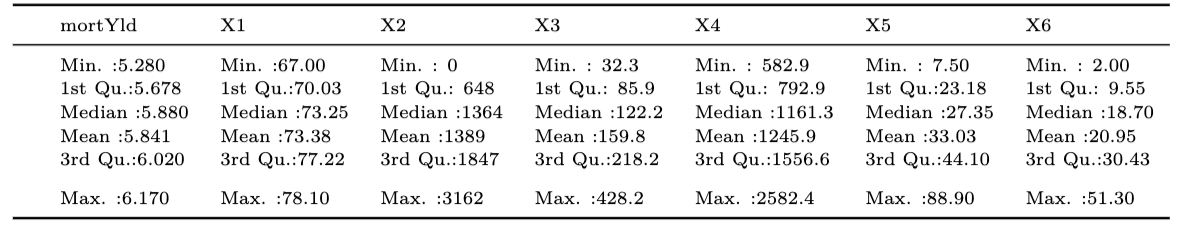
\includegraphics[width=1.0\textwidth]{figures/Table 1.png}
\caption{Table 1: Summary Statistics of Variables}
\end{figure}
\vspace{-0.5cm}

Through this summary, we already observe that Mortgage Yields
(\textbf{mortYld}) don't vary much across regions. Most values are
between 5.2\% and 6.2\%, suggesting relatively stable Mortgage rates.

Loan-to-Mortgage Ratios (\textbf{X1}) are concentrated in between 67\%
and 78.1\%. Distance from Boston (\textbf{X2}) has a vast range (0--3162
miles), highlighting geographical diversity and potential financial
access disparities. Savings per New Unit Built (\textbf{X3}) and Savings
per Capita (\textbf{X4}) are characterized by means bigger than medians,
representing right-skewed distributions. Population Increase
(\textbf{X5}) from 1950 to 1960 varies widely (7.5--88.9\%). Lastly,
Percentage of First Mortgages from Inter-Regional Banks (\textbf{X6})
spans from 2.0\% to 51.3\%, meaning that some areas depend heavily on
external financing while others rely more on local institutions.

\subsubsection{Graphical analysis}\label{graphical-analysis}

\begin{figure}[H]
\centering

\begin{minipage}[t]{0.45\textwidth}
\centering
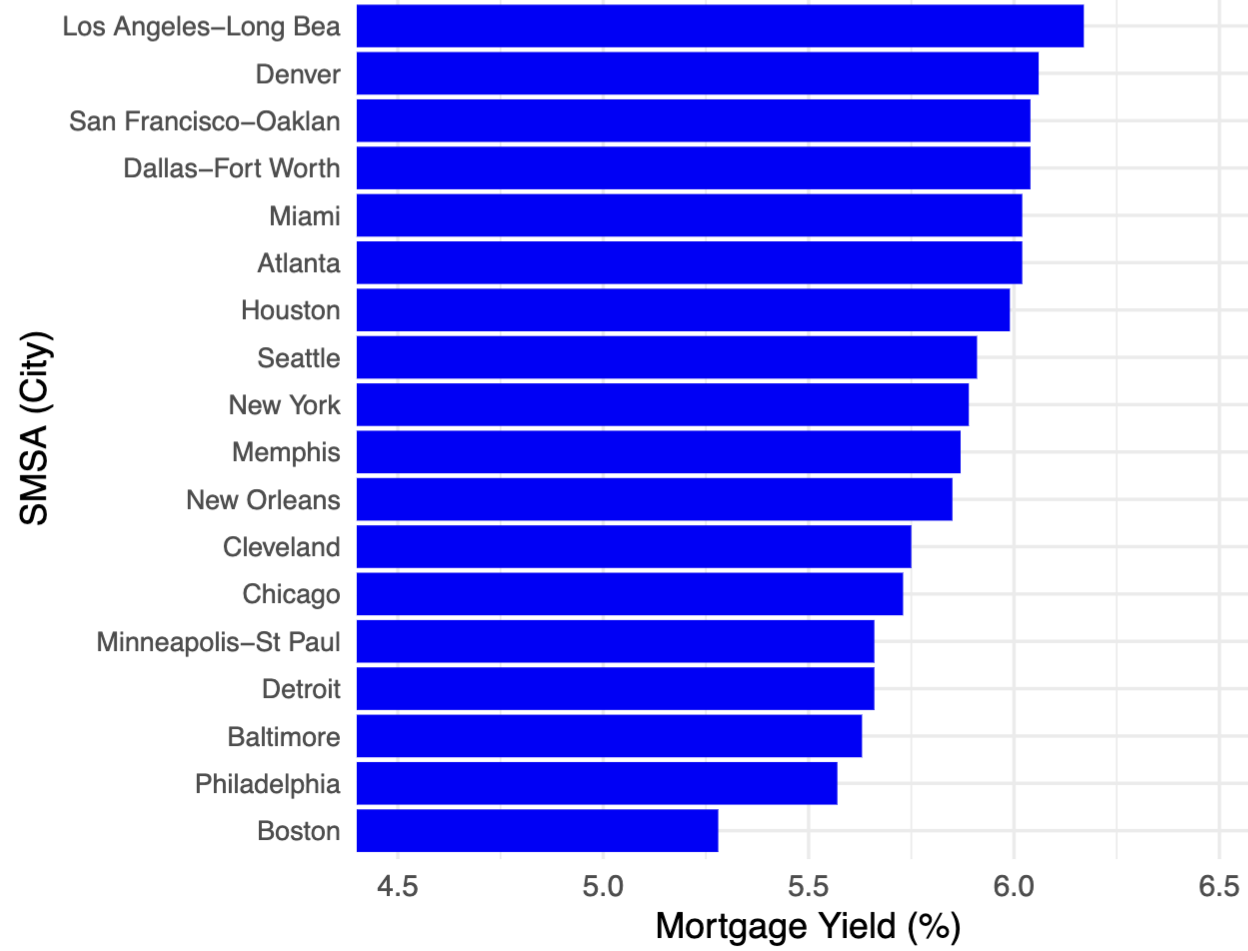
\includegraphics[width=1.1\linewidth]{figures/Figure 1.png}
\caption*{Figure 1: Histogram of Mortgage Yield per SMSA}
\end{minipage}
\hfill
\begin{minipage}[t]{0.45\textwidth}
\centering
\vspace{-6cm}
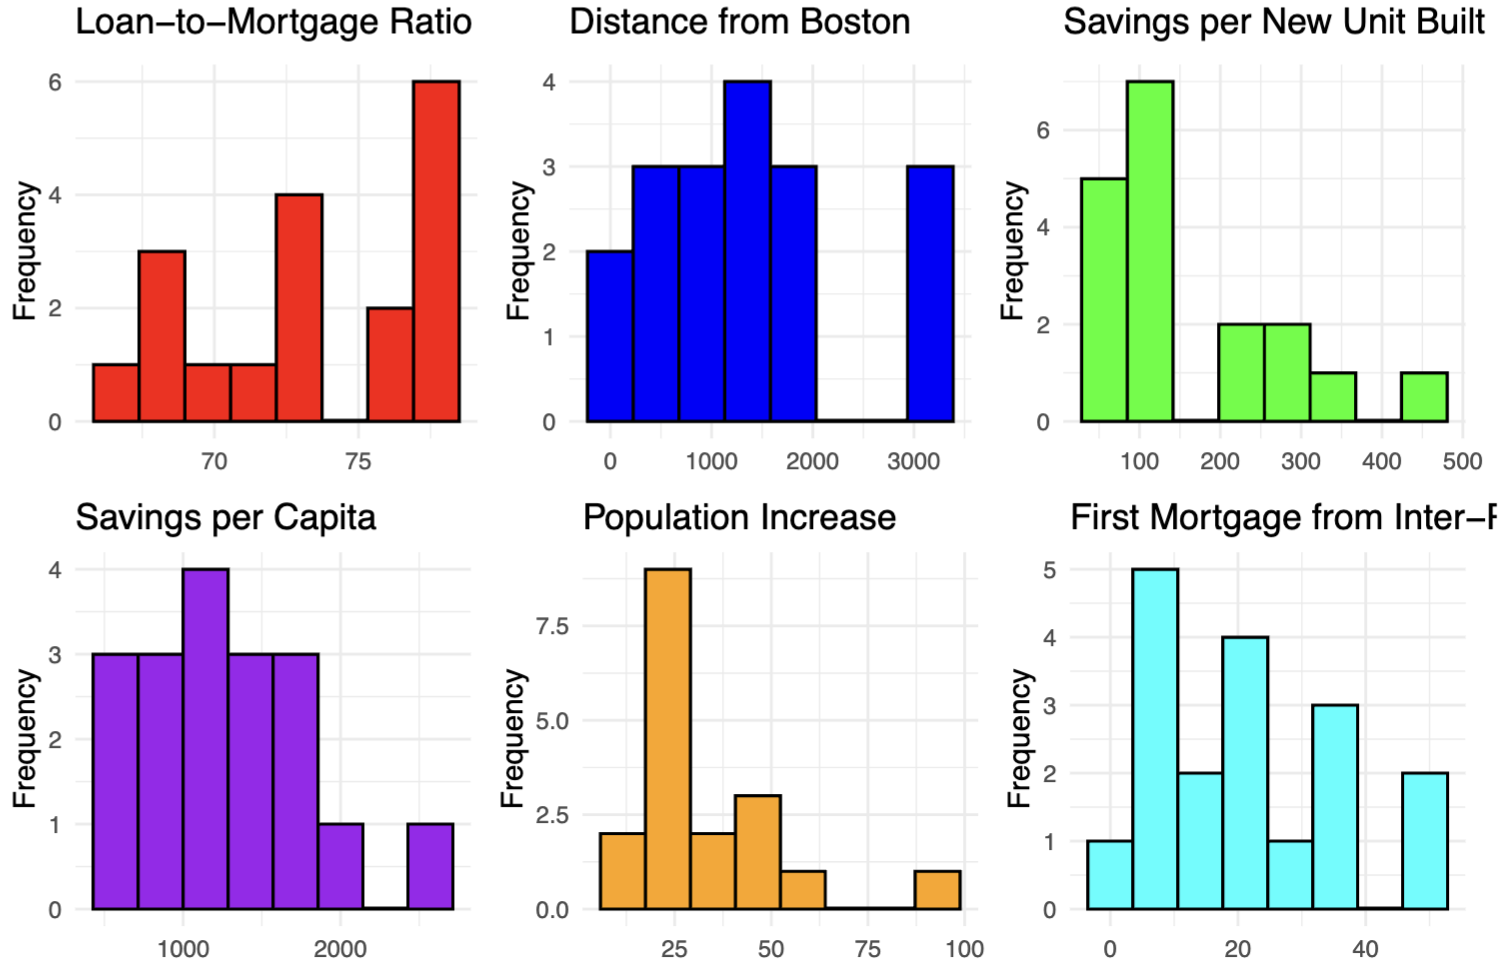
\includegraphics[width=1.1\linewidth]{figures/Figure 2.png}
\caption*{Figure 2: Histograms of each variable (X1 to X6)}
\end{minipage}

\end{figure}
\vspace{-0.5cm}

With deeper analysis, although the variation across SMSAs is small, we
see that regional differences still exist in Mortgage Yields, possibly
due to economic factors like savings, loan terms, and regional banking
practices. The histograms confirm the distribution of the explanatory
variables:

The Loan-to-Mortgage Ratio (\textbf{X1}) shows low variance, possibly
indicating limited variability across regions. Distance from Boston
(\textbf{X2}) displays a wide and almost homogeneous distribution,
reflecting substantial geographic spread among SMSAs. The right-skewed
distributions of Savings per New Unit Built (\textbf{X3}) and Savings
per Capita (\textbf{X4}) suggest that a few cities have notably higher
savings levels. Population Increase (\textbf{X5}) is also highly
right-skewed with one potential major outlier, indicating that most
regions had moderate growth, while a few experienced rapid expansion.
Finally, the percentage of First Mortgages from Inter-Regional Banks
(\textbf{X6}) show that most cities relying minimally on external
financing and a few showing heavy dependence. Overall, the data suggests
regional variation in housing finance conditions, credit accessibility,
and Mortgage market dynamics.

\subsection{Bivariate analysis}\label{bivariate-analysis}

\subsubsection{Graphical analysis}\label{graphical-analysis-1}

The Association Matrix provides a quick visual assessment of bivariate
relationships (how each variable relates to the others and
\texttt{mortYld}), of types of associations among predictors (if a
relationship looks linear, curved or weak, as well as positive or
negative), and of outlier presence. It complements numerical analyses
like the correlation matrix. We can see that most of the plots are
random dispersion, while some are linear, and some are curved.
\textbf{X3} seems to be positively associated with \textbf{X4} and
negatively with \textbf{X5}. \textbf{X2} and \textbf{X3} seem negatively
exponentially associated. \textbf{X6} seems to be negatively associated
with \textbf{X3}.

\begin{figure}[H]
\centering

\begin{minipage}[t]{0.38\textwidth}
\centering
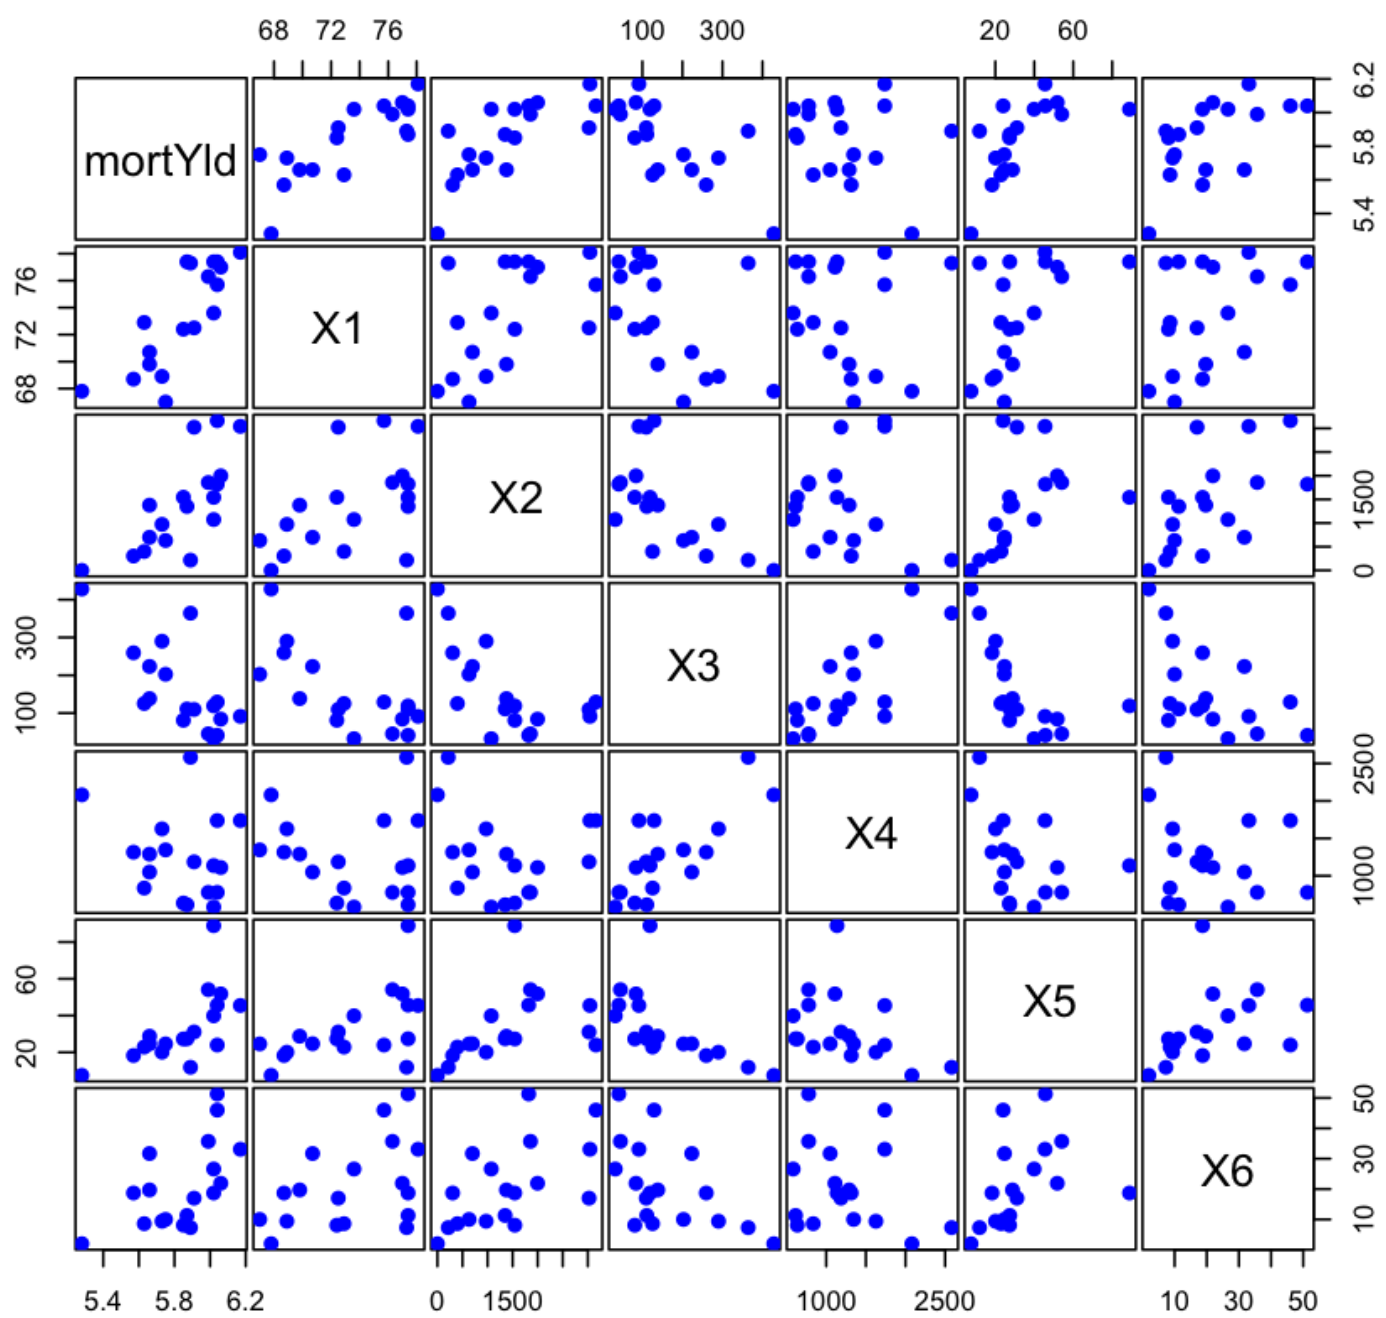
\includegraphics[width=1\linewidth]{figures/Figure 3.png}
\caption*{Figure 3: Association Matrix of Variables and Mortgage Yield}
\end{minipage}
\hfill
\begin{minipage}[t]{0.58\textwidth}
\centering
\vspace{-6cm}
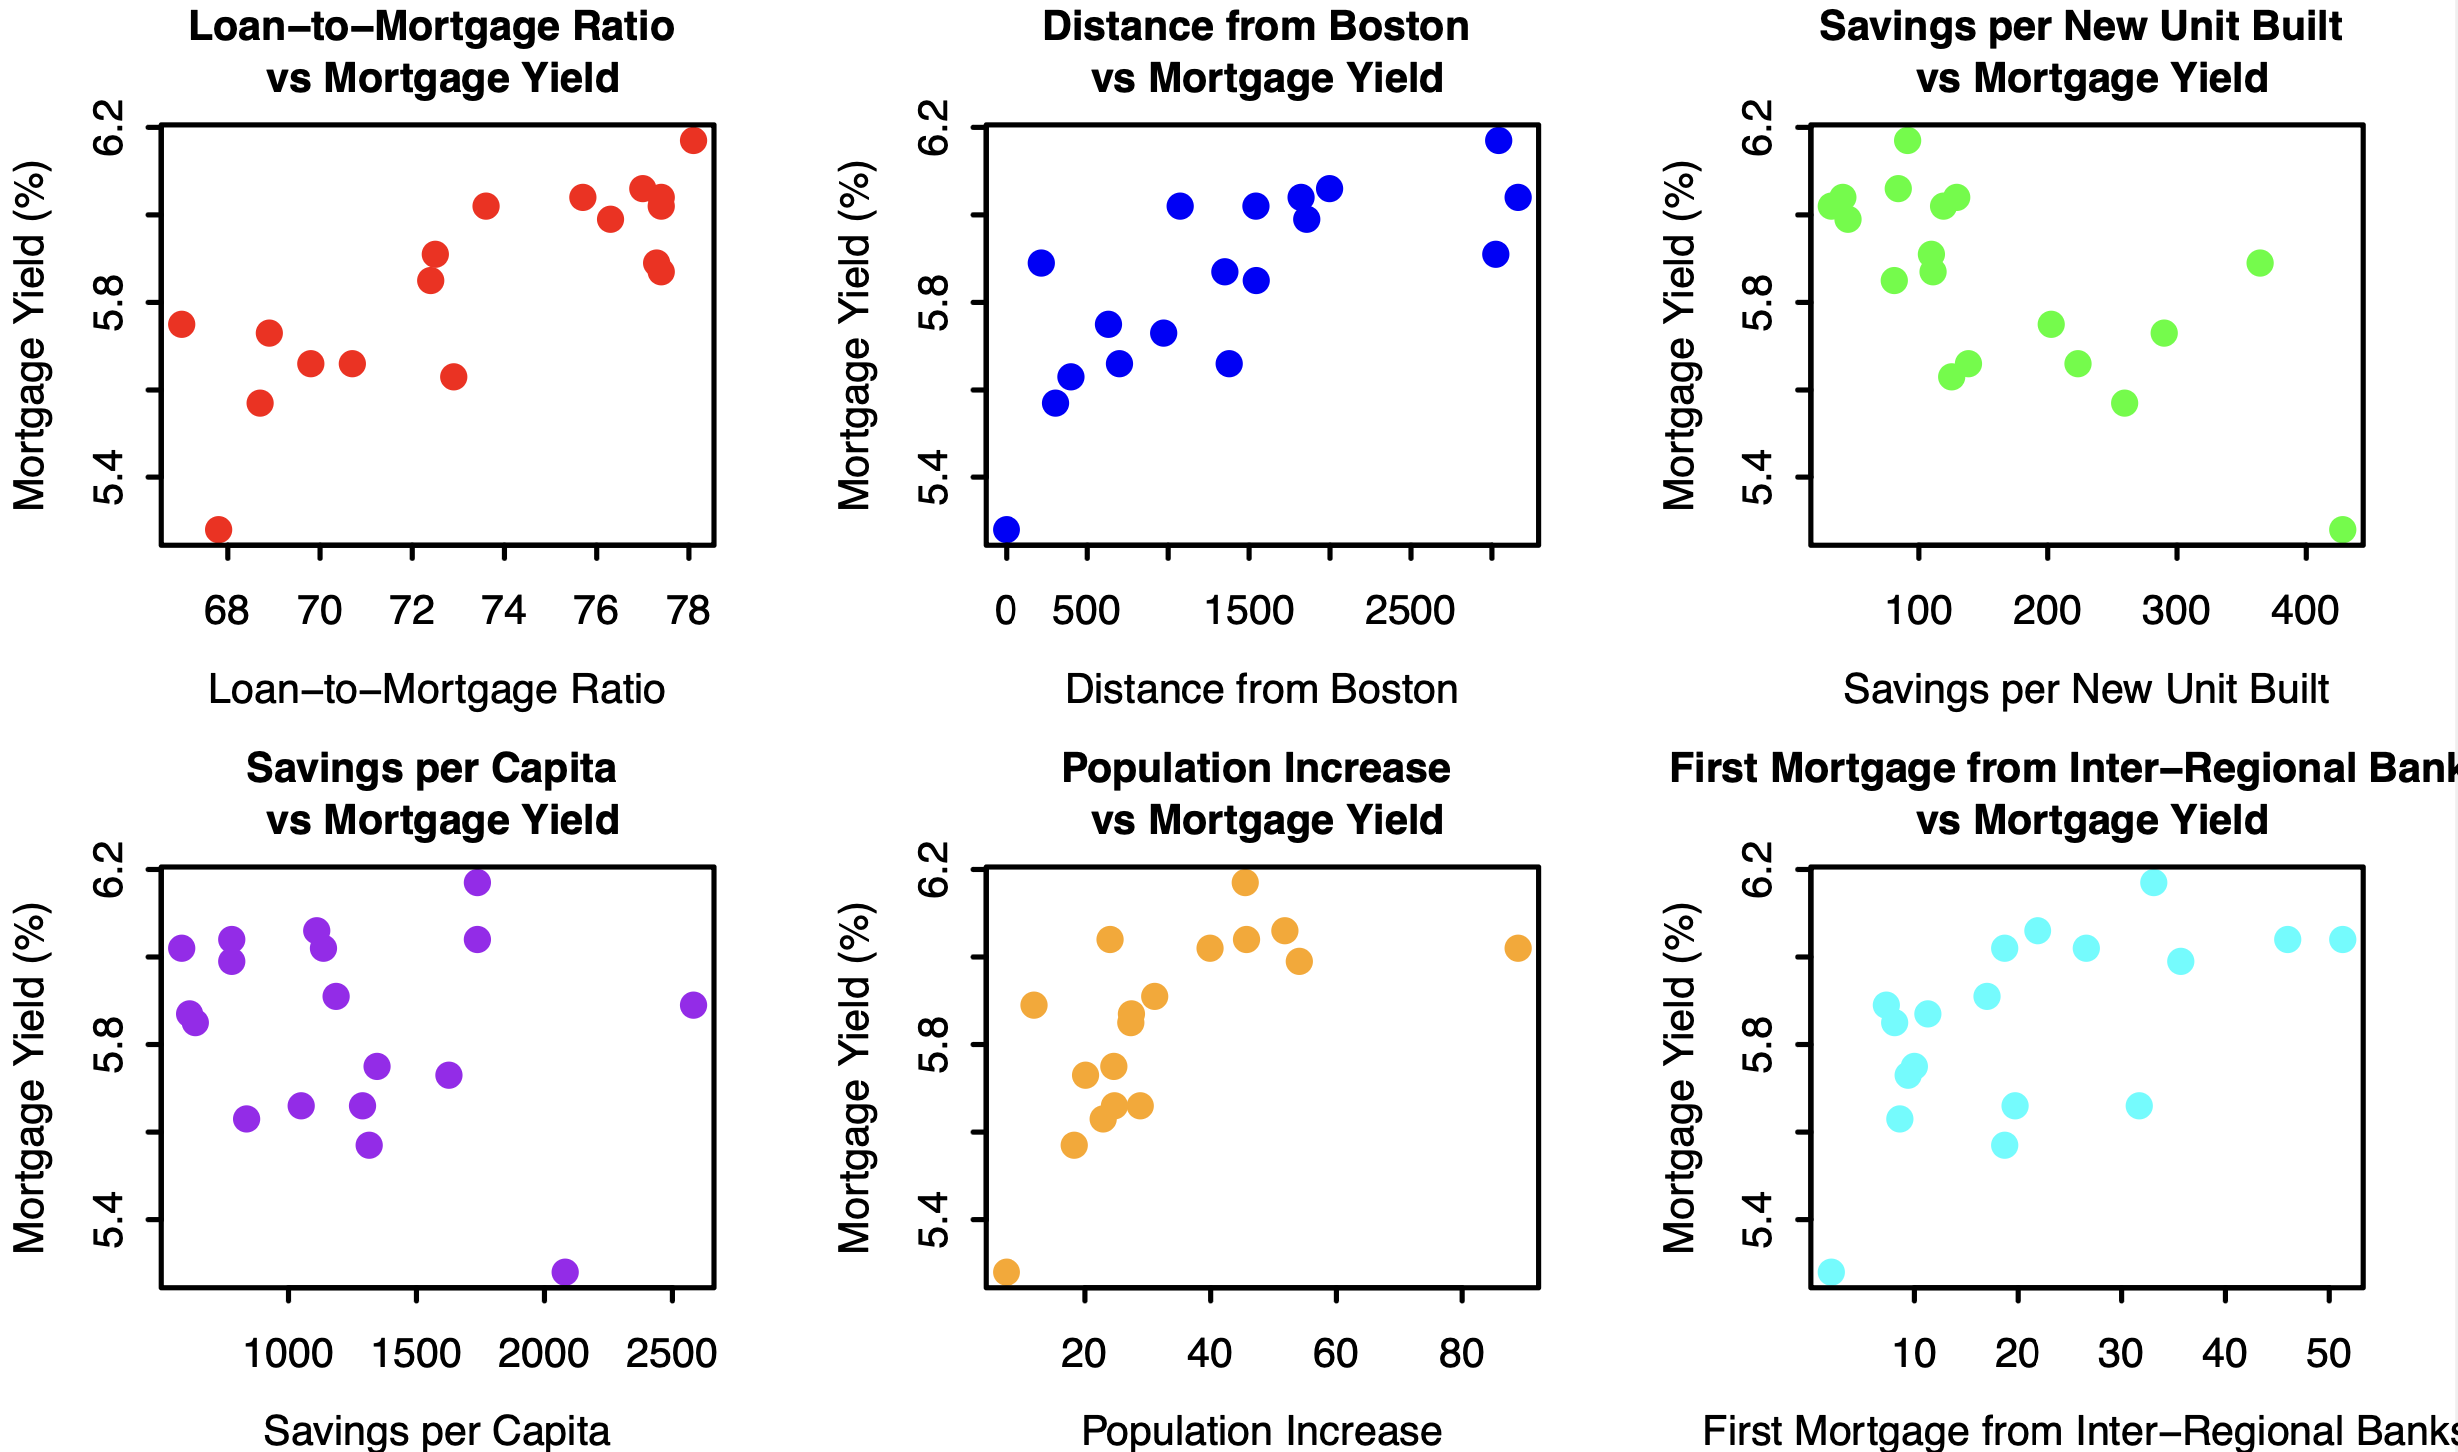
\includegraphics[width=1\linewidth]{figures/Figure 4.png}
\caption*{Figure 4: Scatterplots of each variable (X1 to X6) compared to Mortgage Yield}
\end{minipage}
\end{figure}

Let's take a closer look into the Association Matrix, regarding the
relationship between Mortgage Yield (\%) and the explanatory variables
(x-axis), representing the first row in the precedent figure.\\

As \textbf{X1} increases, the Mortgage Yield increases. This suggests a
positive correlation, and that higher Loan-to-Mortgage Ratios (more
borrowed money relative to the property value) are associated with
higher Mortgage Yields. \textbf{X2} reveals a positive correlation with
\texttt{mortYld}. Boston represents a major financial center with
surplus capital.

Regions further from Boston might have higher Yields. \textbf{X3} seems
to be negatively correlated with \texttt{mortYld}. This indicates that
areas with more savings dedicated to new construction have better access
to local financing, resulting in lower Mortgage Yields. \textbf{X4}'s
influence is less distinguishable but appears to be a weak negative
correlation or a random dispersion. \textbf{X5} shows a positive
association which can be seen as a square-root relationship. High
population growth may imply higher demand for housing, increasing
Mortgage Yields due to heightened competition for available funds. We
can observe a potential outlier at the right side of the plot.
\textbf{X6}'s variation shows no clear trend. It seems like the reliance
on external financing does not significantly influence Mortgage
Yields.\\
These observations support the findings of Schaaf (1966) stating that
distance from financial centers, risk factors, and local demand for
savings contribute to Mortgage Yield variations. \vspace{-3pt}

\subsubsection{Numerical analysis}\label{numerical-analysis-1}

\begin{figure}[H]
\centering
\begin{minipage}{0.39\textwidth}
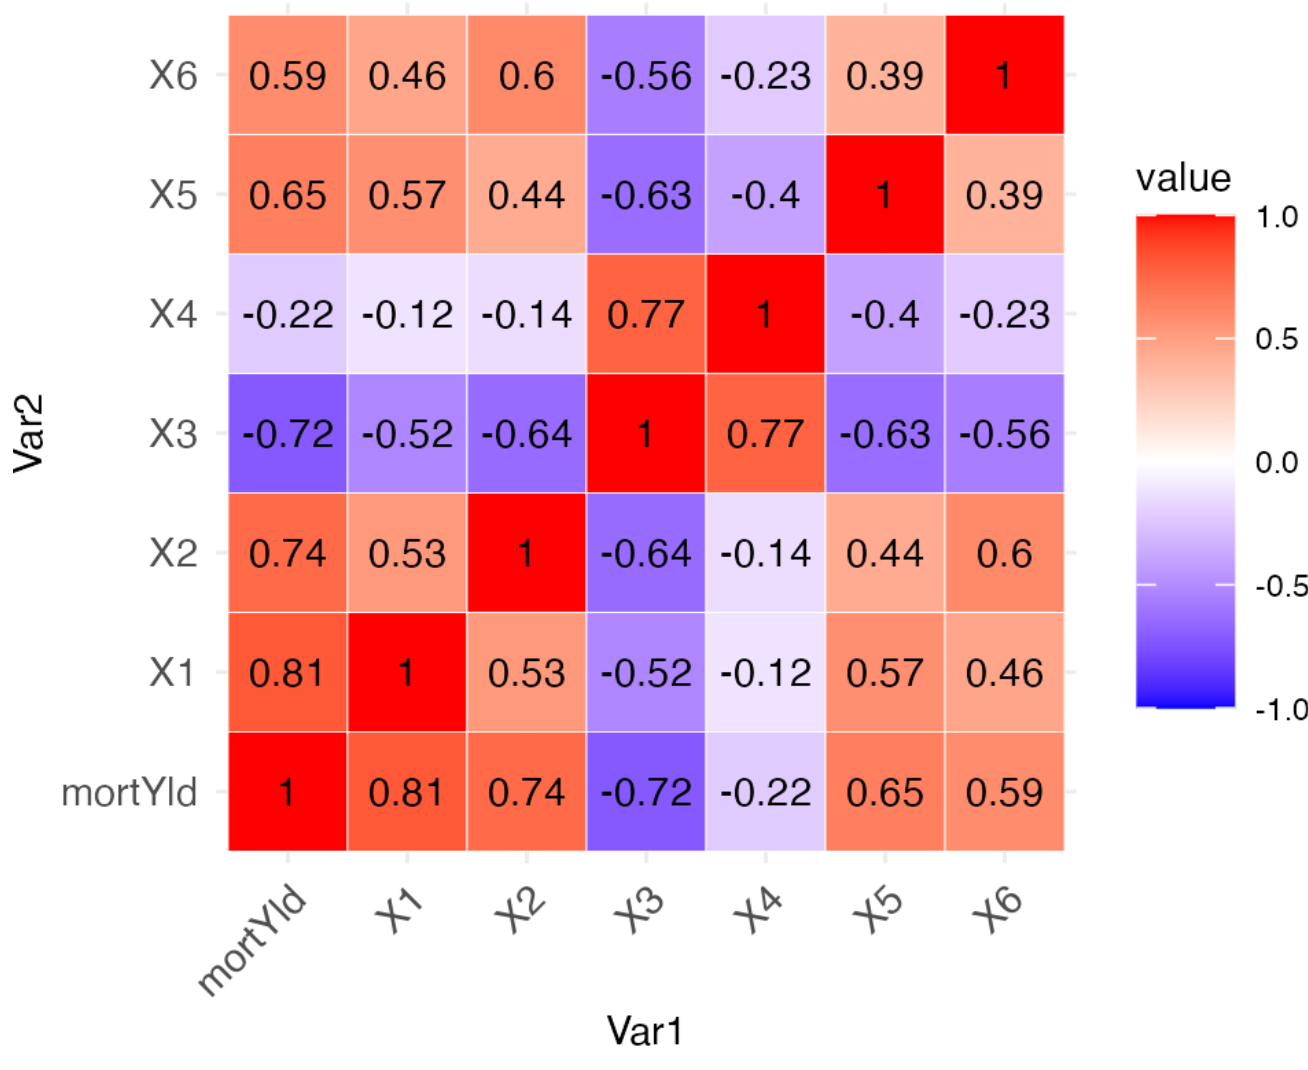
\includegraphics[width=\linewidth]{figures/Figure 5.png}
\caption*{Figure 5: Correlation Heatmaps of variables}
\end{minipage}
\hfill
\begin{minipage}{0.59\textwidth}
\vspace{-1cm}
\small
Now, let's take a look at the correlations between each variable and confirm our previous observations:
\textbf{X3} is strongly positively correlated with \textbf{X4} (0.77) and negatively with \textbf{X2} (-0.64), \textbf{X5} (-0.63), and \textbf{X6} (-0.56).
\textbf{X1} and \textbf{X2} exhibit strong positive correlation with \texttt{mortYld}, while \textbf{X5} shows moderate positive correlation, and \textbf{X3} a strong negative one. \textbf{X6} shows moderate positive correlation with \texttt{mortYld} as well. \textbf{X4} shows only weak correlation with \texttt{mortYld}.


This confirms what we saw earlier in the association matrix.

We can then think about removing one of the highly correlated
predictors, to see if multicollinearity affects the regression model.
However, these correlations only indicate if two variables are linearly
associated. Thus, a low value doesn't necessarily mean that the
variables are not correlated in another way.
\end{minipage}


\end{figure}

\section{Model Fitting}\label{model-fitting}

In this analysis, all predictors are continuous variables and each
observation corresponds to a unique SMSA. Since the dataset contains no
grouping or categorical factors with unequal group sizes, this is a
standard multiple regression model with one observation per row.
Therefore, the design is not factorial and does not involve unbalanced
group structures. As a result, the order of the predictors for the
linear regression model does not influence the coefficient estimates,
F-tests, or model interpretation.

We aim to model the relationship between Mortgage Yield and a set of six
explanatory variables using multiple linear regression.\\
The multiple linear regression model is defined mathematically as:
\vspace{-0.2cm} \[
\text{mortYld}_i = \beta_0 + \beta_1 X_{1i} + \beta_2 X_{2i} + \beta_3 X_{3i} + \beta_4 X_{4i} + \beta_5 X_{5i} + \beta_6 X_{6i} + \varepsilon_i
\] where:\\
• \(\text{mortYld}_i\) is the mortgage yield for the i-th SMSA,\\
• \(X_{1i}\) to \(X_{6i}\) are the explanatory variables,\\
• \(\beta_0\) is the intercept,\\
• \(\beta_1\) to \(\beta_6\) are the regression coefficients,\\
• \(\varepsilon_i\) is the error term for observation i.

\vspace{0.2cm}

We assume the classical linear regression assumptions:\\
1. Linearity: The relationship between each predictor and the outcome is
linear.\\
2. Independence: The errors \(\varepsilon_i\) are independent across
observations.\\
3. Homoscedasticity: The errors have constant variance:
\(\text{Var}(\varepsilon_i) = \sigma^2\).\\
4. Normality: The errors follow a normal distribution:
\(\varepsilon_i \sim \mathcal{N}(0, \sigma^2)\).\\
5. No multicollinearity: The predictors are not perfectly linearly
correlated.

\vspace{0.2cm}

The model is fitted using Ordinary Least Squares (OLS), which minimizes
the sum of squared residuals:\\
\vspace{-0.2cm} \[
\min_{\boldsymbol\beta} \sum_{i=1}^n \left( \text{mortYld}_i - \beta_0 - \sum_{j=1}^6 \beta_j X_{ji} \right)^2
\] \vspace{-0.3cm}

\subsection{Null Model vs Full Model
Comparison}\label{null-model-vs-full-model-comparison}

\vspace{-0.5cm}
\begin{figure}[H]
\centering
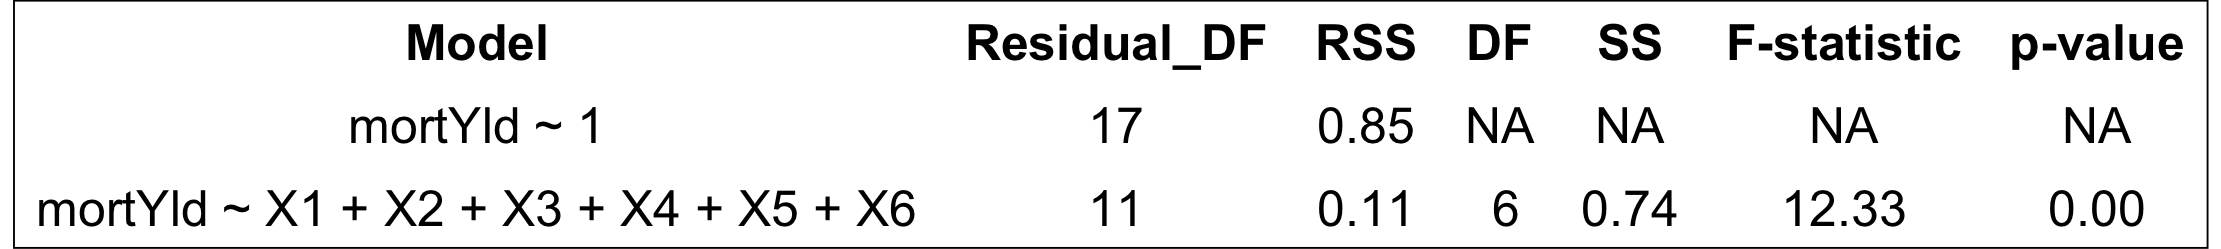
\includegraphics[width=1.0\textwidth]{figures/Table 2.png}
\captionsetup{font=normalsize}
\caption*{Table 4: Comparison of Null and Full Model (ANOVA)}
\end{figure}
\vspace{-0.5cm}

The ANOVA comparison between the null model (intercept-only) and the
full model (including all predictors), reveals that the full model
better explains the Mortgage Yield, as shown by the significant
F-statistic and p-value (p \textless{} 0.001). This indicates that at
least one of the predictors is significantly related to Mortgage Yield.

\begin{minipage}{0.42\textwidth}
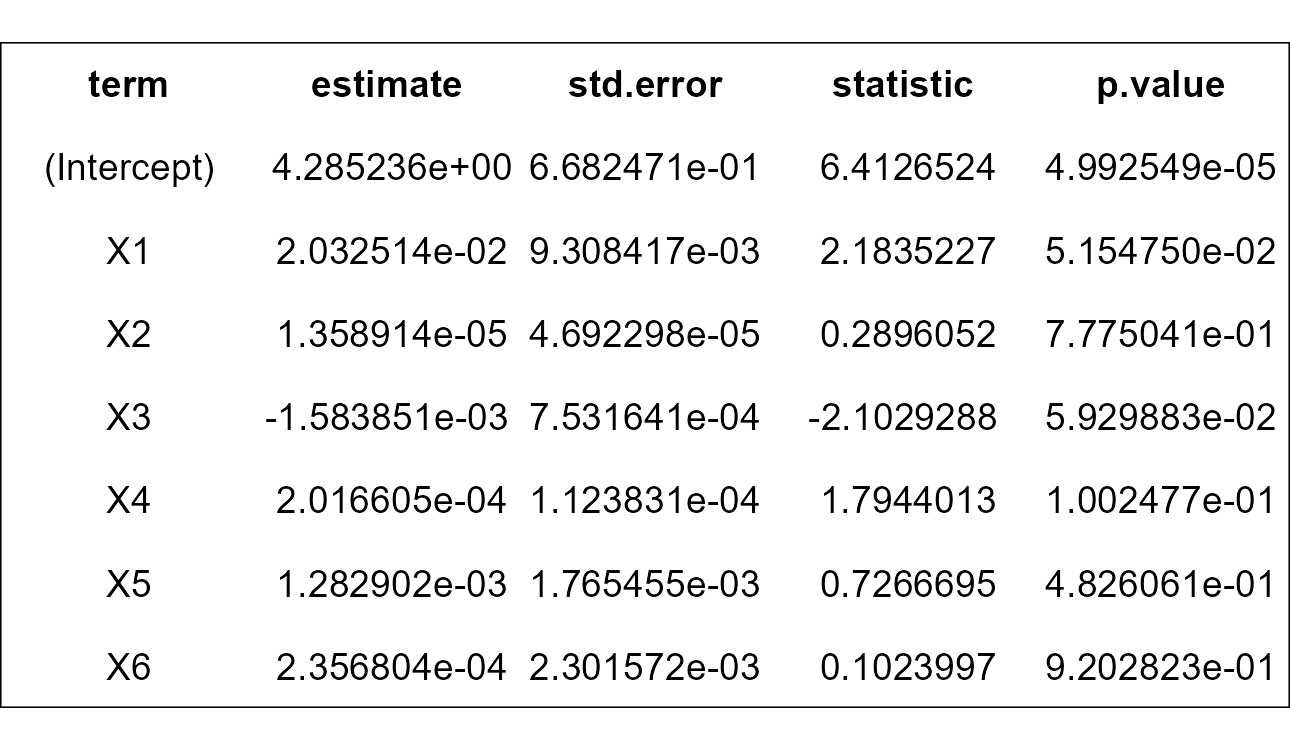
\includegraphics[width=1\linewidth]{full_model_summary_table.png}
\vspace{-0.2em}
{\fontsize{12}{14}\selectfont Table 5: Summary of Full Linear Model}
\end{minipage}
\hfill
\begin{minipage}{0.55\textwidth}
The Full model explains $\sim$87\% of the variance in Mortgage Yield, and 80\% after adjusting for the number of predictors, which highlights a strong fit. The Residual Standard Error is low, and the overall model is statistically significant, with a very low p-value ($p < 0.001$). Once again, it means that at least one term contributes significantly to explaining the variation in \texttt{mortYld}.
\end{minipage}

\noindent \vspace{-5pt}

\begin{figure}[H]
  \centering
  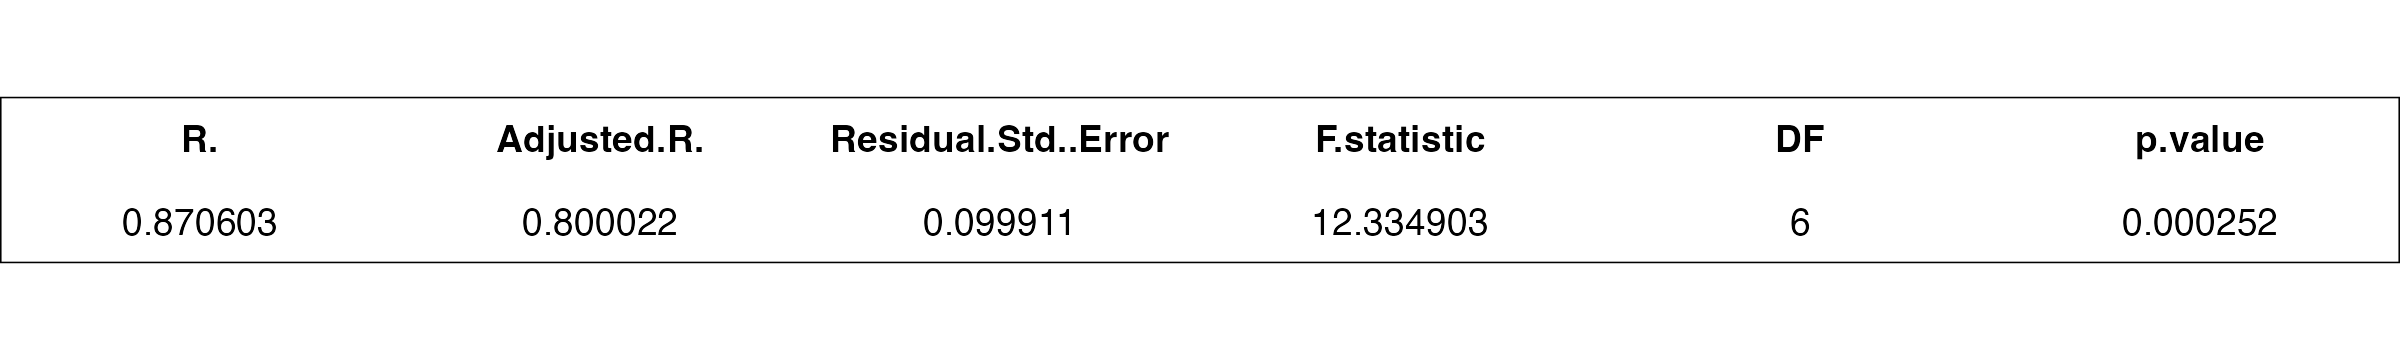
\includegraphics[width=0.9\linewidth, height=0.15\textheight]{full_model_fitstats_table.png}
  \caption*{{\fontsize{12}{14}\selectfont Table 6: Fit Statistics of Full Linear Model}}
\end{figure}
\addtocounter{table}{2}
\vspace{-5pt}

The intercept appears to be strongly significant to fit the model (p
\textless{} 0.001). On the other hand, most of the variables do not show
statistically significant individual contributions: only \textbf{X1} and
\textbf{X3} show weak significance (p \(\approx\) 0.05), while the other
variables, \textbf{X2}, \textbf{X5} and \textbf{X6}, do not show
significant individual effects. This suggests that a reduced model may
be more appropriate.\\
We end up with : \texttt{mortYld} = 4.2852 + 0.0203\(\cdot\)\textbf{X1}
+ 0.0\(\cdot\)\textbf{X2} - 0.0016\(\cdot\)\textbf{X3} +
0.0002\(\cdot\)\textbf{X4} + 0.0013\(\cdot\)\textbf{X5} +
0.0002\(\cdot\)\textbf{X6}

\subsection{Make stepwise regression to select the best
model}\label{make-stepwise-regression-to-select-the-best-model}

\begin{minipage}{0.48\textwidth}
\centering
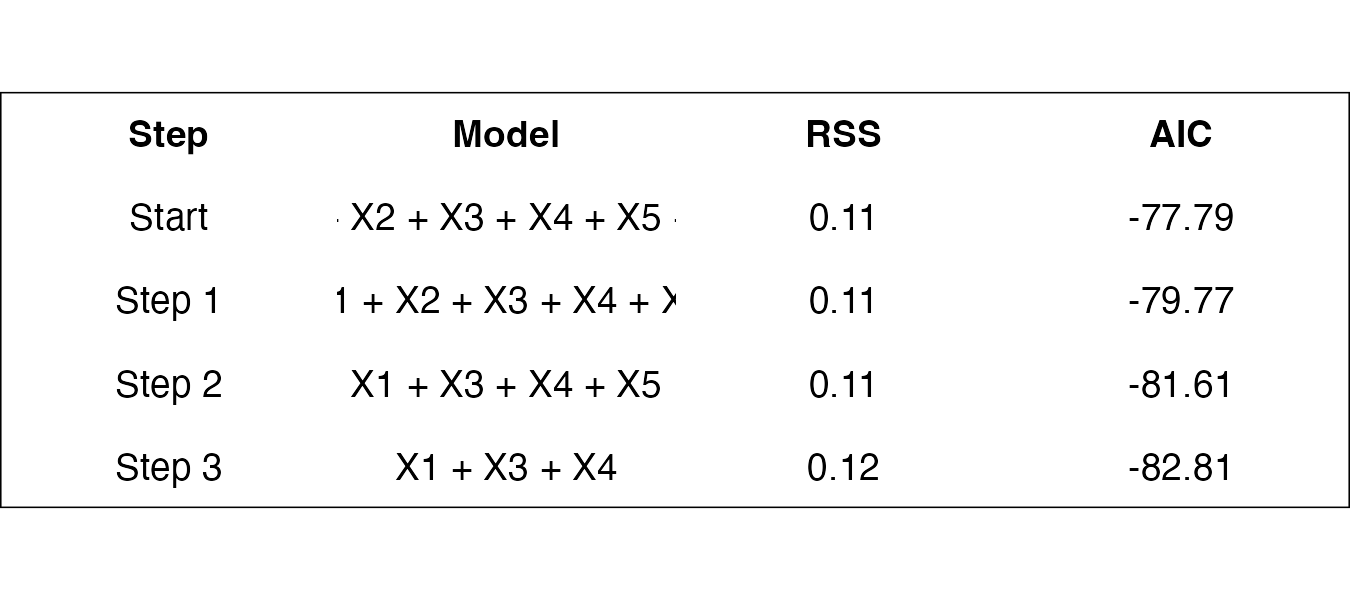
\includegraphics[width=\linewidth]{stepwise_aic_table.png}
\vspace{-2em}
{\fontsize{12}{14}\selectfont Table 7: Stepwise AIC Steps. AIC = Akaike Information Criterion. Lower AIC indicates a better trade-off between model fit and complexity.\par}
\end{minipage}
\hfill
\begin{minipage}{0.48\textwidth}
\centering
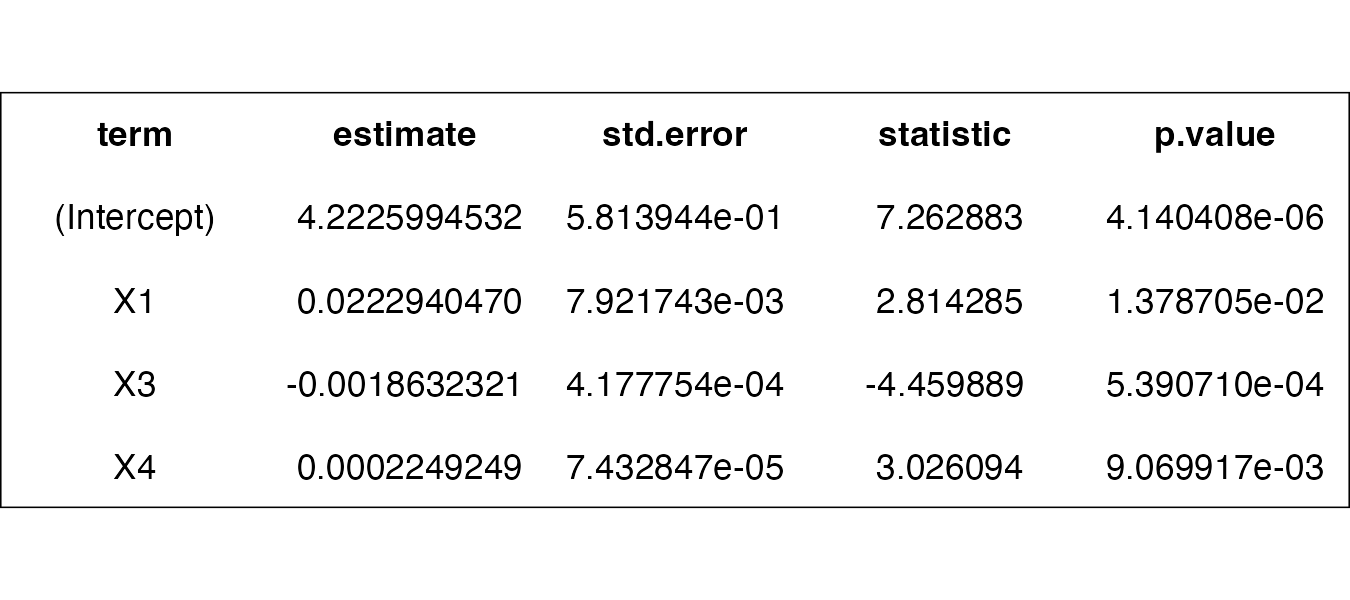
\includegraphics[width=\linewidth]{stepwise_coef_table.png}\\
\vspace{-2em}
{\fontsize{12}{14}\selectfont Table 8: Coefficients of Final Stepwise Model\par}
\end{minipage}

\addtocounter{table}{2}

\begin{table}[!h]
\centering\begingroup\fontsize{8}{10}\selectfont

\begin{tabular}{rrrrrl}
\toprule
$R^2$ & Adjusted $R^2$ & Residual Std. Error & F-statistic & DF & p-value\\
\midrule
0.8634 & 0.8341 & 0.091 & 29.4933 & 3 & 2.62e-06\\
\bottomrule
\end{tabular}
\endgroup{}
\end{table}
\vspace{-2em}
\begin{center}
{\fontsize{12}{14}\selectfont Table 9: Fit Statistics of Stepwise Model\par}
\end{center}

The Stepwise regression process identifies \textbf{X1}, \textbf{X3}, and
\textbf{X4} as the most significant predictors of Mortgage Yield,
constituting the final model.

It is interesting to note that \textbf{X4} appears among the 3 most
significant predictors although it shows very weak correlation in the
Correlation Matrix. Multiple regression measures the effect of each
variable while holding all others constant. As \textbf{X4} has very
strong correlation with \textbf{X3} (0.77), holding \textbf{X3} can make
the unique contribution of \textbf{X4} clearer.

The final Stepwise model explains approximately 83.4\% of the variance
in Mortgage Yield using only these three predictors. The AIC doesn't
increases a lot when keeping more predictors, meaning that even if these
predictors can still be statistically valid to keep, they are not so
useful to the model. Though the final model is simpler, it explains the
data just as well or better than more complex models. The Residual
Standard Error (0.091) is low, and the overall model is highly
significant (p \textless{} 0.001), indicating a good fit.\\
We end up with : \texttt{mortYld} = 4.223 + 0.02229\(\cdot\)\textbf{X1}
- 0.001863\(\cdot\)\textbf{X3} + 0.0002249\(\cdot\)\textbf{X4}\\
\strut \\
Let's now try a model with 2-way interactions.

\begin{minipage}{0.4\textwidth}
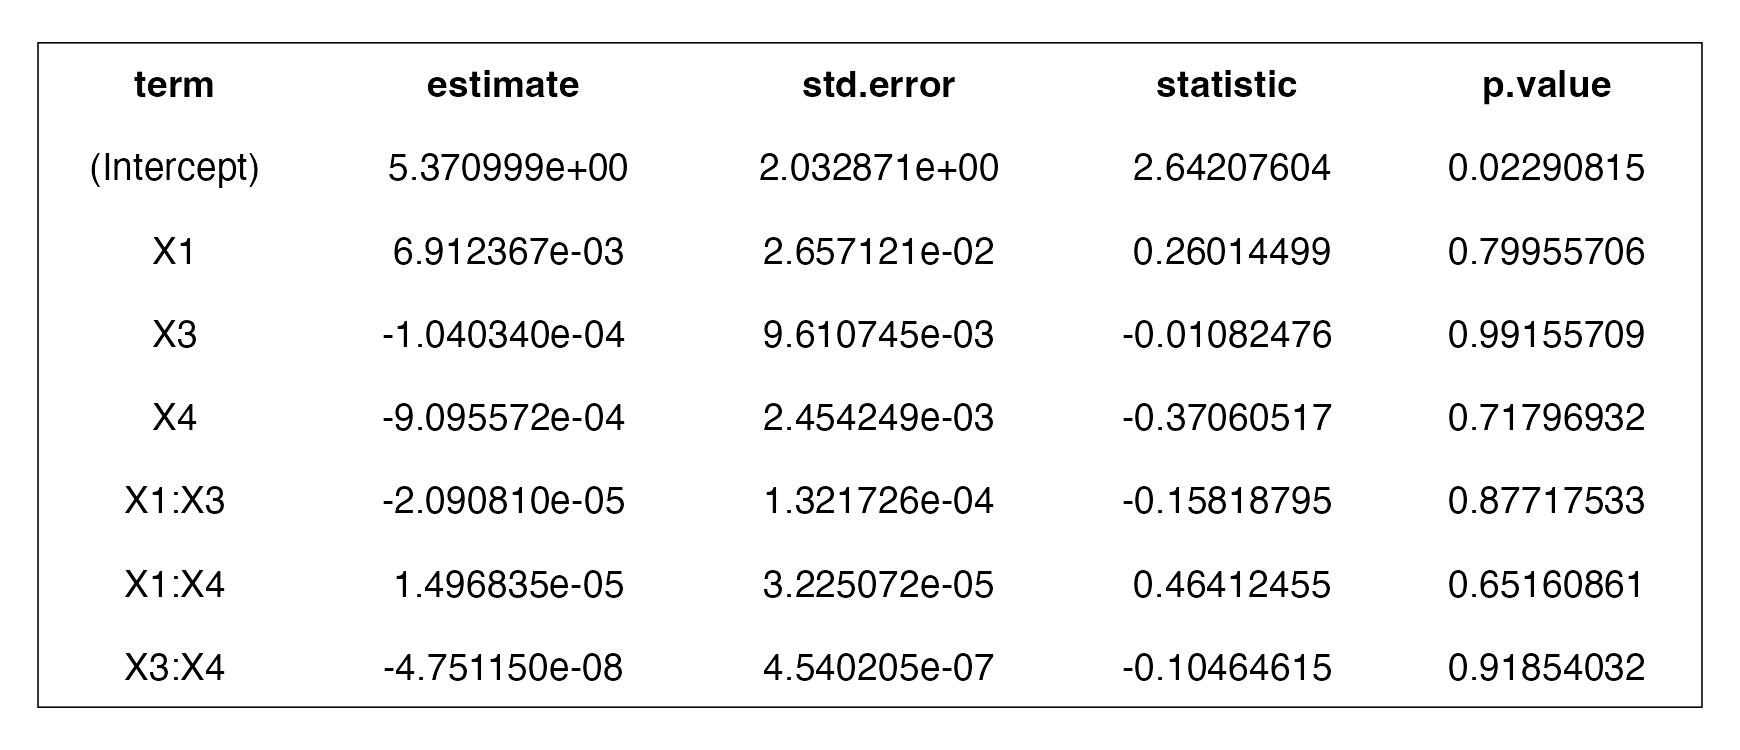
\includegraphics[width=1.5\linewidth]{interaction_model_coef.png}
\vspace{-0.3em}
\fontsize{12}{14}\selectfont Table 10: Coefficients of Interaction Model\par
\end{minipage}
\hfill
\begin{minipage}{0.35\textwidth}
The 2-way Interactions model, which is more complex than the Stepwise
model, explains approximately 79.9\% of the variance in Mortgage Yield.
The Residual Standard Error (0.1002) is low, and the overall model is
highly significant (p < 0.001), indicating that at least one of the
terms has a significant influence on Mortgage Yield.
\end{minipage}

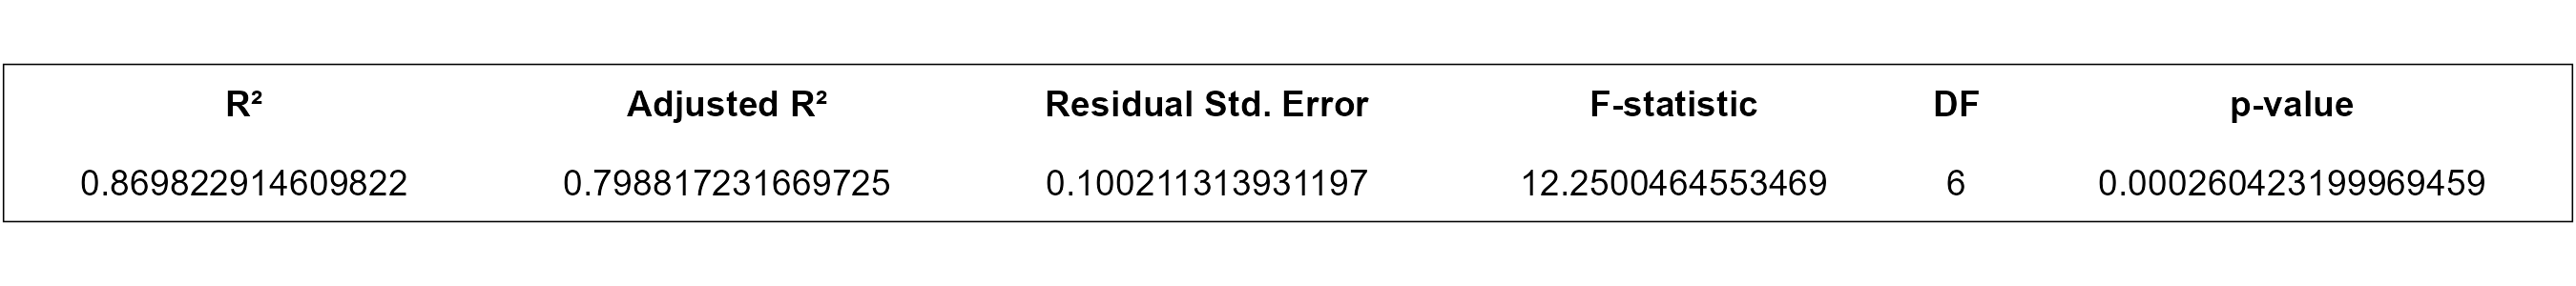
\includegraphics[width=1\linewidth]{interaction_model_fitstats.png}

\par

\fontsize{12}{14}\selectfont Table 11: Fit Statistics of Interaction
Model

\par
\addtocounter{table}{2}

None of the variables show statistically significant individual
contributions: only the intercept appears to be moderately significant
to fit the model (p \textless{} 0.05). This suggests that a reduced
model may be more appropriate.\\
We end up with : \texttt{mortYld} = 5.3710 + 0.0069\(\cdot\)\textbf{X1}
- 0.0001\(\cdot\)\textbf{X3} - 0.0009\(\cdot\)\textbf{X4} +
0.0\(\cdot\)\textbf{X1}:\textbf{X3} +
0.0\(\cdot\)\textbf{X1}:\textbf{X4} +
0.0\(\cdot\)\textbf{X3}:\textbf{X4}\\
\strut \\
We decided not to include a 3-way Interactions model in our analysis.
Given the small sample size (18 observations), adding high-order
interactions would significantly reduce degrees of freedom and increase
the risk of overfitting. Moreover, 3-way interactions are often
difficult to interpret meaningfully.

\subsection{Model Comparison}\label{model-comparison}

\begingroup\fontsize{8}{10}\selectfont

\begin{longtable}[t]{lrrrrr}
\caption{\label{tab:unnamed-chunk-9}Comparison of Model Performance Metrics}\\
\toprule
Model & R2 & Adj\_R2 & AIC & Residual\_SE & F\_statistic\\
\midrule
Full Model & 0.87 & 0.80 & -24.71 & 0.10 & 12.33\\
Stepwise Model & 0.86 & 0.83 & -29.73 & 0.09 & 29.49\\
2-Way Interaction Model & 0.87 & 0.80 & -24.60 & 0.10 & 12.25\\
\bottomrule
\end{longtable}
\endgroup{}

The Stepwise model offers the best trade-off between simplicity and
performance: it has the lowest AIC (\textasciitilde29.7), demonstrating
the best model fit among the three. Despite having a slightly lower R²
than the Full and 2-ways Interactions model, it achieves the highest
Adjusted R². It also has the lowest Residual Standard Error (0.091) and
the highest F-statistic (\textasciitilde29.5). This confirms the overall
model significance and parsimony.

\begin{table}[!h]
\centering
\caption{\label{tab:unnamed-chunk-10}ANOVA Comparison: Stepwise vs Interactions Model}
\centering
\fontsize{8}{10}\selectfont
\begin{tabular}[t]{lrrrrrr}
\toprule
Model & Res.Df & RSS & Df & Sum of Sq & F & Pr(>F)\\
\midrule
Stepwise model & 14 & 0.12 & NA & NA & NA & NA\\
Interaction model & 11 & 0.11 & 3 & 0.01 & 0.18 & 0.91\\
\bottomrule
\end{tabular}
\end{table}

An ANOVA is then conducted to compare the Stepwise Model and the
Interaction Model, which are nested --- the Interaction Model extends
the Stepwise Model by including additional two-way interaction terms.
The test yields an F-statistic of 0.18 and a p-value of 0.91, indicating
that the additional interaction terms do not significantly reduce the
residual variance. As a result, the simpler model with only main effects
(\textbf{X1}, \textbf{X3}, and \textbf{X4}) truly provides the best fit,
as it also offers comparable explanatory power and better
interpretability.

\section{Model assumptions and
Diagnostics}\label{model-assumptions-and-diagnostics}

\subsection{Independence evaluation}\label{independence-evaluation}

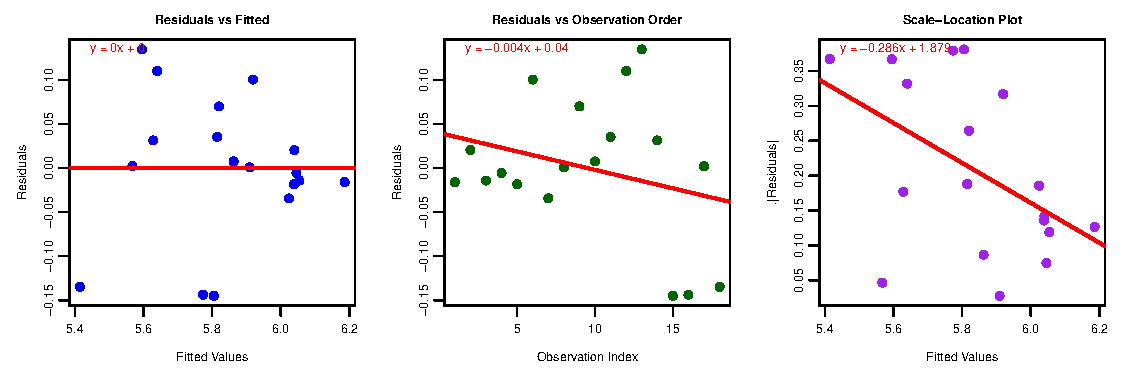
\includegraphics{Figs/unnamed-chunk-11-1.pdf}

The \texttt{Residuals\ VS\ Fitted\ Values} plot shows that the residuals
are randomly scattered around 0, with no clear pattern. This suggests
that the assumptions of linearity and constant error variance are
reasonably met. Secondly, the slightly negative but close to zero slope
(-0.286) in the \texttt{Scale-Location\ Plot} indicates that the spread
of residuals is almost constant across fitted values. This is a sign
that our model doesn't suffer from heteroscedasticity and is likely a
good fit: homoscedasticity seems therefore satisfied.

The \texttt{Residuals\ VS\ Observation\ Order} plot helps us conclude
that there is no consistent trend: the independence of residuals is
verified, as they are not correlated with the order of observations.

\vspace{-0.5em}

\subsection{Multicolinearity
diagnostic}\label{multicolinearity-diagnostic}

\noindent

\begin{minipage}{0.75\textwidth}
\vspace{-0.5em}
As all variables have a VIF value under 5, it means that they don’t cause problematic multicollinearity in the final model and that none of them should be eliminated. This confirms our choice of keeping \textbf{X3} and \textbf{X4}: even if they showed a high correlation coefficient (0.77), these variables still provide enough unique, non-redundant information to justify keeping them in the model.
\end{minipage}
\hfill
\begin{minipage}{0.2\textwidth}
\vspace{-3em}
  \begin{figure}[H]
    \centering
    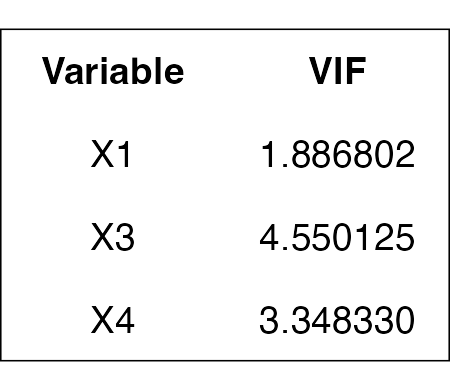
\includegraphics[width=0.8\linewidth]{vif_table.png}
    \vspace{-0.5em}
    \captionsetup{font=normalsize}
    \caption*{Table 14: Variance Inflation Factors (VIF)}
  \end{figure}
\end{minipage}

\vspace{-1em}

\subsection{Normality Check}\label{normality-check}

\noindent

\begin{minipage}{0.65\textwidth}
\justifying
\vspace{-3.5em}
The \texttt{Q-Q plot of Residuals} indicates that most of the points align closely with the 45-degree line, suggesting that the residuals are approximately normally distributed. However, six points deviate at the extremes of the theoretical quantiles, which indicates the presence of potential outliers or heavy tails in the distribution. In a dataset with just 18 observations, small deviations in the Q-Q plot are usual. Outliers or deviations are common in such a small sample size and do not automatically suggest a violation of normality.
\end{minipage}
\hfill
\begin{minipage}{0.33\textwidth}
\centering
\vspace{-2em}  % Reduce space before image
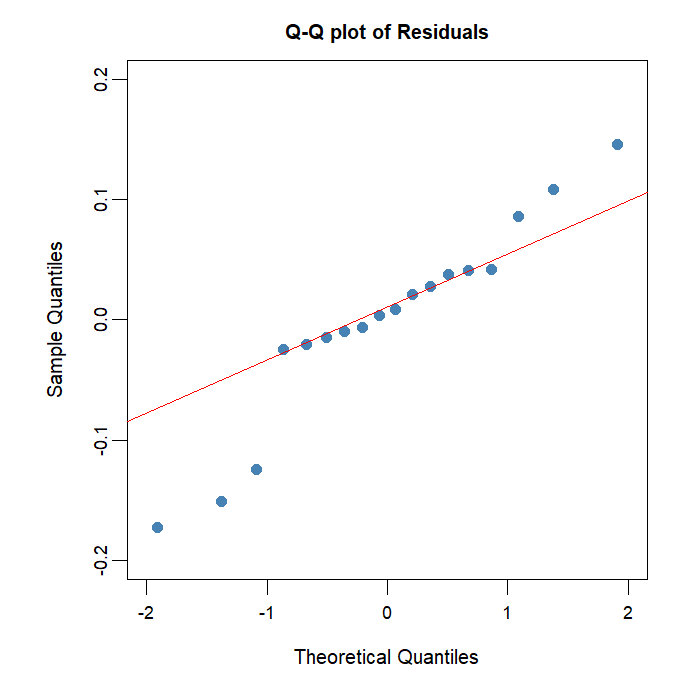
\includegraphics[width=0.9\linewidth]{qqplot_residuals.png}
\vspace{-1em}     % Reduce space after image
\end{minipage}

\vspace{-3em}

\section{Conclusion}\label{conclusion}

The final estimated model is : \texttt{mortYld} = 4.223 +
0.02229\(\cdot\)\textbf{X1} - 0.001863\(\cdot\)\textbf{X3} +
0.0002249\(\cdot\)\textbf{X4}\\
where \textbf{X1} is the Loan-to-Mortgage Ratio, \textbf{X3} is the
Savings per New Unit Built, and \textbf{X4} is the Savings per Capita.

The analysis shows that these variables significantly impact Mortgage
Yield. Mortgage Yield is positively influenced by the Loan-to-Mortgage
Ratio, indicating that higher loan amounts relative to mortgages may
lead to better returns for lenders. Conversely, Mortgage Yield is
negatively impacted by Savings per New Unit Built, suggesting that more
capital saved for construction could reduce reliance on mortgages,
leading to lower returns. Finally, Savings per Capita has a positive,
though small, effect on Mortgage Yield. As individual savings increase,
it may signal a more financially stable environment, leading to slightly
better mortgage performance.

While the assumptions of linear regression are generally satisfied,
there are some minor deviations. The model shows strong predictive
performance, accounting for 83.4\% of the variance in Mortgage Yield,
with homoscedasticity nearly achieved.

Future improvements could include exploring additional predictors,
testing for non-linear relationships, or refining the model to better
capture any residual heteroscedasticity.

\end{document}
